\subsection{Redes neuronales artificiales. Proceso de cálculo hacia delante.}

Las redes neuronales son algoritmos que se usan en el campo de la Inteligencia Artificial y tratan solventar problemas en los cuales se trabaja con gran cantidad de datos tratando de buscar patrones en ellos. Además, es una de las pocas alternativas a otros algoritmos que nos son capaces de tratar gran volumen de datos. 
\newline

Los inicios de las redes neuronales se remontan a la década de 1950, cuando McCulloch y WalterPitts\cite{kleene} trabajaron en un modelo matemático que se asemejaba al comportamiento que conocían de una neurona. El ciéntifico Frank Rosenblatt, inspirado en este trabajo, desarrollo lo que se conoce como redes de perceptrones. Este fue el primer acercamiento a lo que hoy se conoce como redes neuronales\cite{nielsen}. 

\subsubsection{Perceptrón}
Un perceptrón, o neurona es una unidad básica de inferencia en forma de discriminador lineal, es la base de lo que se conoce hoy como neurona artificial\cite{nielsen}. Básicamente, un perceptrón toma varios valores binarios como entrada $x_1, x_2, …, x_n$ y produce un único valor de salida $y$.
\newline

\begin{figure}[H]
    \centering
    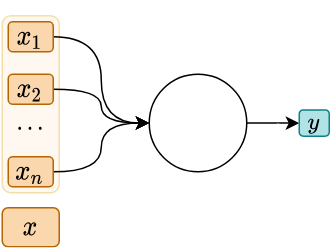
\includegraphics[width=6cm]{images/state-of-art/perceptron/perceptron.png}
    \caption{Representación del funcionamiento de un perceptrón}
    \label{fig:perceptronprocess}
\end{figure}

Además del vector $x$ y el valor $y$, el perceptron tiene dos componentes más: 
\begin{itemize}
    \item El vector de pesos $w$ que expresa la importancia de las respectivas entradas para la salida y tendrá el mismo número de elementos que $x$. Este vector se usará para calcular la suma ponderada  $\sum_i w_ix_i$.
    \item El umbral o sesgo (\textit{bias}($b$) en inglés): El valor del sumatorio se comprobará si es menor o mayor a este valor $b$. En función de ello, el valor $y$ será $0$ o $1$. El umbral es un valor que representa lo fácil que es producir un valor $1$ en $y$. Para un perceptrón con un sesgo muy grande, es extremadamente fácil que el perceptrón produzca un $1$. Pero si el sesgo es muy negativo, entonces es difícil que el perceptrón produzca un $1$.
\end{itemize}

Tanto el vector $w$ y el valor umbral $b$ son parámetros que se deben de saber previamente. El valor $y$ producido por el perceptrón viene dado por la siguiente ecuación: 

\begin{eqnarray}
  y & = & \left\{ \begin{array}{ll}
      0 & \mbox{si } \sum_i w_i x_i \leq b \\
      1 & \mbox{si } \sum_i w_i x_i > b
      \end{array} \right.
      \label{eqn:perceptroncomplex}
\end{eqnarray}


Visto gráficamente:
\begin{figure}[H]
    \centering
    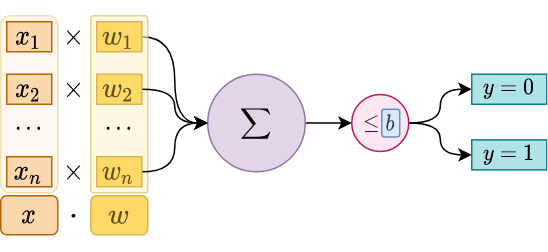
\includegraphics[width=8cm]{images/state-of-art/perceptron/perceptron_weights.png}
    \caption{Representación de un perceptrón}
    \label{fig:perceptron}
\end{figure}

Simplificando la ecuación \ref{eqn:perceptroncomplex} usando el producto vectorial y cambiando de lado $b$:
\begin{eqnarray}
  y & = & \left\{ \begin{array}{ll}
      0 & \mbox{si } w \cdot x + b \leq 0 \\
      1 & \mbox{si } w \cdot x + b > 0
      \end{array} \right.
      \label{eqn:perceptron}
\end{eqnarray}

Visto gráficamente:
\begin{figure}[H]
    \centering
    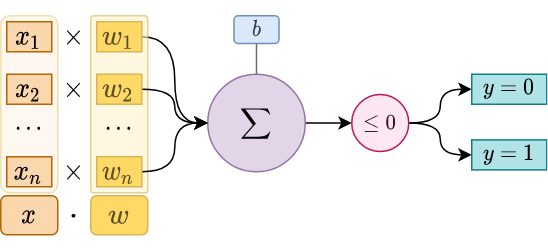
\includegraphics[width=8cm]{images/state-of-art/perceptron/perceptron_weights_complex.png}
    \caption{Representación de un perceptrón}
    \label{fig:perceptron}
\end{figure}


Los perceptrones se pueden agrupar formando capas y estas capas se pueden agrupar a su vez formando una red. Se puede ver el funcionamiento de una red neuronal programando una puerta lógica XOR que recibe dos argumentos binarios de entrada y emite una salida como se puede ver a continuación:
\begin{table}[H]
\centering
\begin{tabular}{| c | c | c |}
\hline
A & B & Salida \\
\hline
$x_1$ & $x_2$ & $y$ \\
\hline
0 & 0 & 0 \\
0 & 1 & 1\\
1 & 0 & 1\\
1 & 1 & 0\\
\hline
\end{tabular}
\caption{Puerta lógica XOR}
\end{table}

Una red neuronal que actúa como una puerta XOR es la siguiente:
\begin{figure}[H]
    \centering
    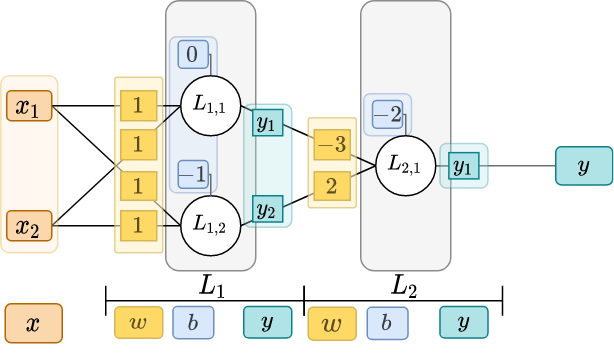
\includegraphics[width=11cm]{images/state-of-art/perceptron/xor.png}
    \caption{Red de perceptrones programada para una puerta lógica XOR}
    \label{fig:xorgatenetwork}
\end{figure}

Las redes se suelen representar con un grafo ponderado unidireccional. El grafo está dividido por capas, en este caso en dos capas ($L_1$ y $L_2$). Cada capa tiene como mínimo una neurona, que será representada por $L_{l,i}$ siendo $l$ el número de la capa e $i$ el índice de la neurona dentro de la capa. 
\newline

Los valores de los pesos se representan como si fuesen los pesos de las aristas. La cantidad de pesos que tendrá una capa asociada a ella viene dada por la multiplicación del número de neuronas en la capa $L_{l}$ por el número de neuronas en la capa anterior $L_{l-1}$. Por último, cada neurona tendrá asociado un valor $b$ que será representado como un término independiente conectado a la neurona por una línea. Por ejemplo, la neurona $L_{2,1}$ tiene asociado el vector $w = [3, -2]$ y el valor $b = -2$.
\newline

Con el grafo ya explicado, se resuelve a continuación el problema que se había planteado: Programar una puerta lógica XOR con una red neuronal. Esta red recibe recibe dos valores binarios de entrada y devolverá un único valor binario. A modo de ejemplo se realizan los cálculos para distintos ejemplos:
\begin{eqnarray}
    Para &\boxed{x = (0, 0)} \nonumber\\
    y^{L_{1,1}} & \implies & \begin{pmatrix}1&1\end{pmatrix} \cdot x^T + 0 = 0 \implies y^{L_{1,1}} = 0 \nonumber\\
    y^{L_{1,2}} & \implies &\begin{pmatrix}1&1\end{pmatrix} \cdot x^T - 1 = -1 \implies y^{L_{1,2}} = 0 \nonumber \\
    y = y^{L_{2,1}} & \implies &\begin{pmatrix}3&-2\end{pmatrix} \cdot \begin{pmatrix}0\\0\end{pmatrix} - 2= -2 \implies \boxed{y = 0} \nonumber \\ \nonumber \\
    Para &\boxed{x = (0, 1)} \nonumber\\
    y^{L_{1,1}} & \implies &\begin{pmatrix}1&1\end{pmatrix} \cdot x^T + 0 = 1 \implies y^{L_{1,1}} = 1\nonumber\\
    y^{L_{1,2}} & \implies &\begin{pmatrix}1&1 \end{pmatrix} \cdot x^T - 1 = 0 \implies y^{L_{1,2}} = 0\nonumber\\
    y = y^{L_{2,1}} & \implies &\begin{pmatrix}3&-2\end{pmatrix} \cdot \begin{pmatrix}1\\0\end{pmatrix} - 2 = 1 \implies \boxed{y = 1}\nonumber \\ \nonumber \\
    Para &\boxed{x = (1, 1)} \nonumber\\
    y^{L_{1,1}} & \implies &\begin{pmatrix}1&1\end{pmatrix} \cdot x^T + 0 = 2 \implies y^{L_{1,1}} = 1\nonumber\\
    y^{L_{1,2}} & \implies &\begin{pmatrix}1&1 \end{pmatrix} \cdot x^T - 1 = 1 \implies y^{L_{1,2}} = 1\nonumber\\
    y = y^{L_{2,1}} & \implies &\begin{pmatrix}3&-2\end{pmatrix} \cdot \begin{pmatrix}1\\1\end{pmatrix} - 2 = -1 \implies \boxed{y = 0}\nonumber \\ \nonumber
\end{eqnarray}

\subsubsection{Regresión lineal}


En realidad, la arquitectura de la red en la figura \ref{fig:xorgatenetwork} usa una neurona que tiene como objetivo simular una puerta lógica OR ($L_{1,1}$) y otra neurona una puerta lógica AND ($L_{1,2}$). Viendo la lógica de una puerta XOR:
\begin{eqnarray}
    A \oplus B = (A \land \neg B) \lor (\neg A \land B) = (A \lor B) \land (\neg A \lor \neg B)
\end{eqnarray}

Tiene sentido que se usen las puertas OR y AND en la red. Se puede ver gráficamente el funcionamiento de cada neurona en la siguiente imagen:
\begin{figure}[H]
    \centering
    
\includegraphics[width=15cm]{images/state-of-art/regression/xor.png}
    \caption{Puertas lógicas OR($L_{1,1}$), AND($L_{1,2}$) y XOR($L_{2,1}$)}
    \label{fig:orandxorgraph}
\end{figure}

Cada una de estas neuronas está realizando una tarea de clasificación, simplemente comprueba si los datos de entrada se encuentran en un lado o en otro de la recta. Esto es así porque se ha definido el perceptrón de tal forma que solo pueda devolver $0$ o $1$. Pero eliminando ese paso de clasificación que se ha definido en la ecuación \ref{eqn:perceptron}, se obtendría una regresión lineal tal que:
\begin{eqnarray}
  y = w \cdot x + b
      \label{eqn:neuronsimple}
\end{eqnarray}

Una regresión lineal es el otro tipo de tarea que una neurona puede resolver. Esta es una de las principales diferencias entre las neuronas modernas y los perceptrones. Los perceptrones solo están programados para realizar una tarea de clasificación, pero las neuronas se pueden programar para otro tipo de casos. Aunque como se explicará posteriormente, un perceptrón es un tipo de neurona con una función de activación escalonada (ver apartado \ref{activationfunction}).
\newline

\begin{figure}[H]
    \centering
    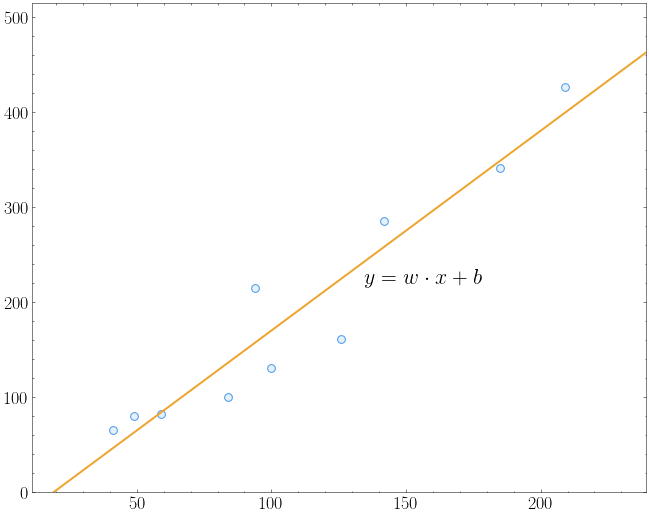
\includegraphics[width=9cm]{images/state-of-art/regression/regression.png}
    \caption{Ejemplo de regresión lineal en un espacio bidimensional}
    \label{fig:regression}
\end{figure}

Una regresión lineal es un método que estudia la relación existente entre varias variables y de ese modo genera un modelo que puede ser usado para estimar otros valores. Matemáticamente, en un espacio multidimensional $n$, una regresión se define de la siguiente manera:
\begin{eqnarray}
  y = w_0 + w_1x_1 + w_2x_2 + ... + w_nx_n
  \label{linealregression}
\end{eqnarray}


En esta ecuación hay un término independiente $w_0$, y por cada dimensión, habrá un valor $w$ y un valor $x$ asociado a ella. Geométricamente, en un espacio de dos dimensiones, $z$ será una recta, un plano si si son tres dimensiones y un hyperplano para mayores de tres dimensiones, que gráficamente no se puede representar. De hecho, se puede observar que la ecuación \ref{eqn:neuronsimple} es en realidad la función de una recta, siendo $b$ el término independiente. 
\newline

A partir de este punto se usará $z$ para referirse a la regresión lineal que es calculada en una neurona:
\begin{equation}
  z \equiv y = w \cdot x + b
  \label{eqn:z_equation_init}
\end{equation}

% Un ejemplo visual para mostrar la regresión lineal podría ser el siguiente. Usando $b=0.5$, la recta que quedaría sería:

% TODO AÑadir imagen con colores azul y rojo

% Añadir nota: La zona en azul sería la zona, donde $y=0$ y la zona en verde donde $y=1$. 
% \newline




\subsubsection{Función de activación}\label{activationfunction}

Lo anterior, se puede comprobar matemáticamente que el efecto de sumar muchas operaciones de regresión lineal equivale a una única regresión lineal. Esto se demuestra en la sección \ref{feedforward}. El perceptrón que se ha creado puede colapsar hasta ser equivalente a tener una única neurona. Para evitar esto, debemos calcular valores que no den como resultado una función lineal(una línea recta en dos dimensiones), necesitamos que cada una de estas neuronas aplique alguna función para realizar algún tipo de manipulación no lineal que distorsione sus valores de salida y para ello se usan las funciones de activación \cite{nielsen}.
\newline

A modo de ejemplo, se mostrará con un ejemplo con un modelo con solo funciones lineales comparado con un modelo que usa funciones no lineales. Para ello, se expone el siguiente ejemplo: se quiere crear un modelo de regresión que trate de predecir el valor de una función seno. Al ser el seno una función no lineal, se necesitará de funciones no lineales para resolver el problema.

\begin{equation}
    y = \sin(x)
\end{equation}

También se mostrará código para ir introduciendo el funcionamiento de las librerias que se usan popularmente en mundo del \textit{machine learnig}. Como se explica en SECCION TODO, en este trabajo se han usado \verb|keras|(redes neuronales), \verb|numpy|(vectores y matrices) y \verb|matplotlib|(representar funciones) entre otras. 
\newline

Como se explica en la sección de entrenamiento(sección \ref{training}), se necesita un dataset para que la red se pueda entrenar. El dataset se creará de la siguiente forma:


\begin{minted}[fontsize=\footnotesize]{python}
# real sen data
x = np.linspace(0, 2*np.pi, 1000)
y = np.sin(x)

# some noise is added to the real dataset to make it 
# look like a real world data set
noise = 0.1
noisex = x + np.random.normal(-noise, noise, 1000)
noisey = y + np.random.normal(-noise, noise, 1000)
\end{minted}

Gráficamente quedaría una serie de puntos esparcidos alrededor de la función seno como es de esperar:
\begin{figure}[H]
    \centering
    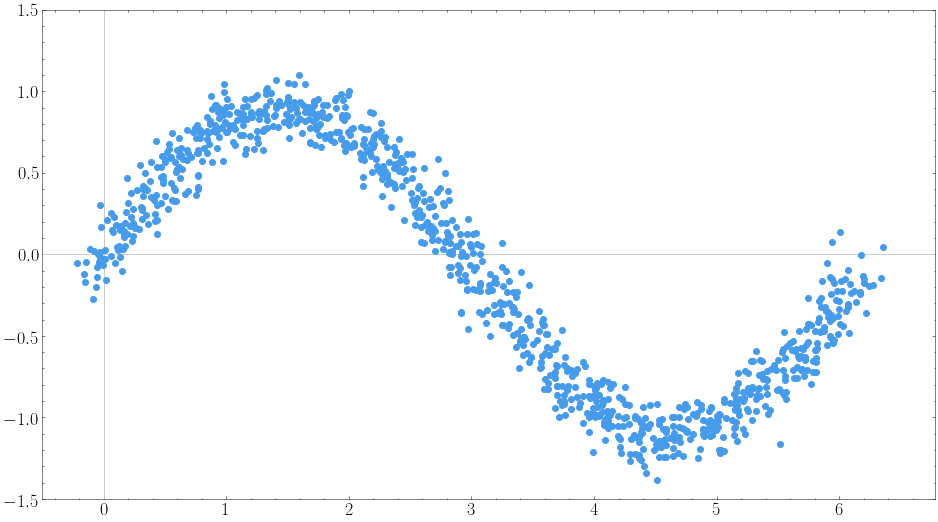
\includegraphics[width=11cm]{images/state-of-art/activation-functions/sin.png}
    \caption{Dataset emulando una función seno}
    \label{fig:basicneuron}
\end{figure}

Se crearán dos modelos, es decir, dos redes con arquitecturas distintas: Un modelo con funciones de activación lineales(\verb|linear_model|) y otro con funciones de activación no lineales(\verb|relu_model|).
\newline

El primer modelo viene definido de la siguiente forma:

\begin{minted}[fontsize=\footnotesize]{python}
linear_model = Sequential()
linear_model.add(Dense(32, activation='linear'))
linear_model.add(Dense(32, activation='linear'))
linear_model.add(Dense(1))
\end{minted}

Lo que se hace en ese código es crear la arquitectura de la red. Será una red con tres capas densas. Las dos primeras capas son las capas ocultas del modelo y se indica que se quieren 32 neuronas en cada capa con la función de activación \verb|linear|. La última capa simplemente es para que el modelo solo devuelva un único valor.
\newline

La otra red usará una función no lineal de activación ReLU, explicada posteriormente. EL código para la arquitectura de esta red es la siguiente:
\begin{minted}[fontsize=\footnotesize]{python}
relu_model = Sequential()
relu_model.add(Dense(32, activation='relu'))
relu_model.add(Dense(32, activation='relu'))
relu_model.add(Dense(1))
\end{minted}

Posteriormente se "compila" el modelo. En este paso, se indicará a \textit{keras} que se parámetros tanto obligatorios como opcionales se quieren para red. Estos parámetros serán explicados en próximas secciones. Justo después se entrena a los modelos.
\begin{minted}[fontsize=\footnotesize]{python}
# Compile linear model
linear_model.compile(loss='mean_squared_error', 
                     optimizer='adam')
# Train linear model
linear_model.fit(noisex, noisey, epochs=100, verbose=0)

# Compile ReLU model
relu_model.compile(loss='mean_squared_error',
                   optimizer='adam')
# Train ReLU model
relu_model.fit(noisex, noisey, epochs=100, verbose=0)
\end{minted}

Para realizar una predición con estos modelos simplemente se puede usar la función \verb|predict()| del modelo:
\begin{minted}[fontsize=\footnotesize]{python}
predicted_by_linear = linear_model.predict(x)
predicted_by_relu = relu_model.predict(x)

# Plot predictions
plt.plot(x, predicted_by_linear)
plt.plot(x, predicted_by_relu)
\end{minted}

\begin{figure}[H]
    \centering
    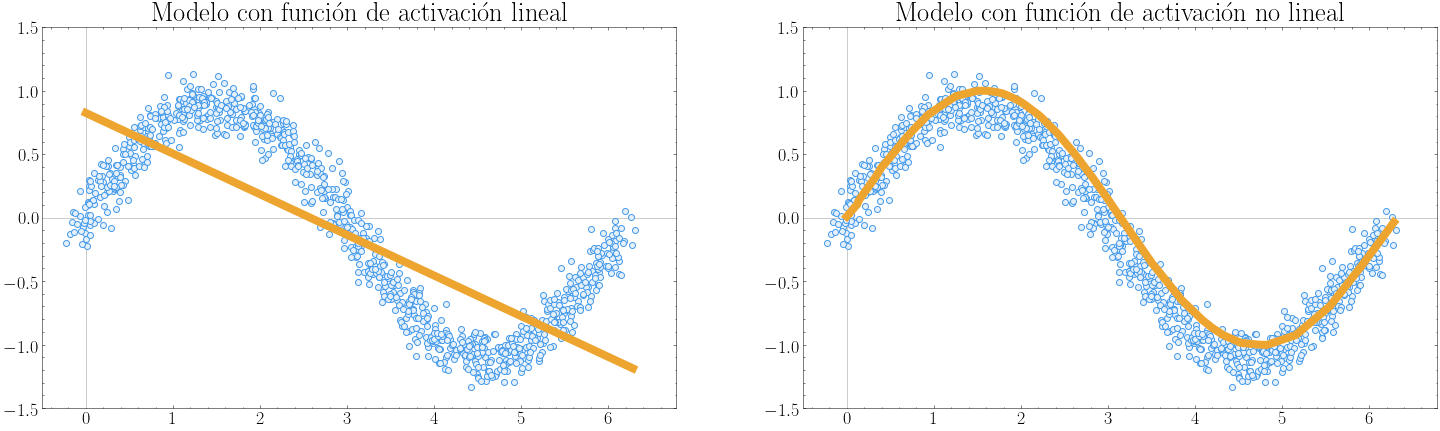
\includegraphics[width=15cm]{images/state-of-art/activation-functions/sin_activation_function.png}
    \caption{Comparativa de funciones de activación lineal y no lineal}
    \label{fig:basicneuron}
\end{figure}

Como se puede observar, el modelo que usa una función de activación lineal se reduce a una única recta mientras que el modelo que usa una función de activación no lineal se adapta correctamente.
\newline

En resumen, la función de activación es una función que se aplica al resultado de la suma ponderada de los valores de entrada, es decir, a $z$. El objetivo es que distorsione el resultado de la neurona añadiéndole deformaciones no lineales para que así se pueda encadenar de forma efectiva la computación de varias neuronas. Se representará esta función de activación de la siguiente forma:

\begin{equation}
    a(z) = a(w \cdot x + b)
    \label{eqn:activationfunctionbasic}
\end{equation}

Actualizando la imagen que se ha usado antes para definir un perceptrón, quedaría tal que:
\begin{figure}[H]
    \centering
    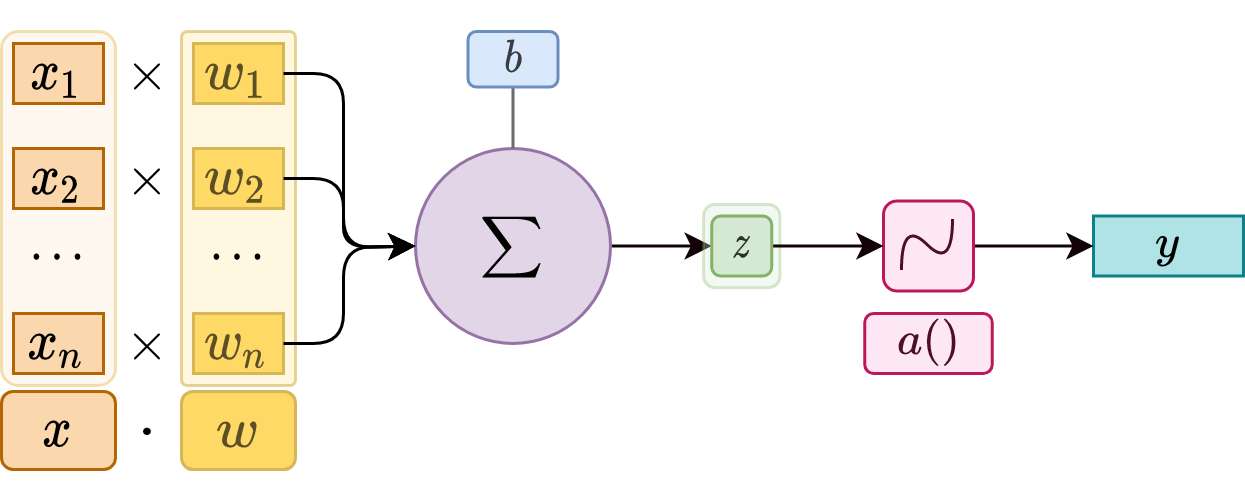
\includegraphics[width=10cm]{images/state-of-art/activation-functions/activation_representation.png}
    \caption{Representación de funcionamiento de una neurona}
    \label{fig:basicneuron}
\end{figure}

Existen varios tipos de función de activación, estas son las más usadas:

\begin{itemize}
\item Lineal: Es simplemente la ecuación de una recta y por lo tanto una función lineal. Normalmente se utiliza en la última capa en un modelo de regresión, es decir, un modelo que realiza una tarea de regresión y no una tarea de clasificación.
\begin{eqnarray}
  a(z) & = & z \\
  a'(z) & = & 1 
\end{eqnarray}

\item Escalonada (\textit{step} en inglés): El objetivo de la función es convertir los valores a $0$ o a $1$ en función de $b$. El propósito de esta función de activación es imitar una neurona que "se activa" o "no se activa" basándose en la información de entrada. Tradicionalmente, esta función se usaba en las redes de perceptrones y de hecho, es la usada en la ecuación \ref{eqn:perceptroncomplex}. La ecuación es la siguiente:

\begin{eqnarray}
  a(z) & = & \left\{ \begin{array}{ll}
      0 & \mbox{si } z \leq 0 \\
      1 & \mbox{si } z > 0
      \end{array} \right. \\
     \newline
  a'(z) & = & 0 
\end{eqnarray}


\item Rectificada lineal (ReLU): Es una función lineal cuando es positiva y constante a 0 cuando el valor es negativo. Es muy usada porque es una función no lineal y parecida a la función lineal, por lo que es rápido de computar.

\begin{eqnarray}
    a(z) & = & max(0,z) \\
  a'(z) & = & \left\{ \begin{array}{ll}
      0 & \mbox{si } z \leq 0   \\
      1 & \mbox{si } z > 0 
      \end{array} \right.
\end{eqnarray}

Existe una variante de esta función de activación (conocida como \textit{leaky}). En esta variante, se cambia la inclinación a un valor $s$ de la parte negativa respecto al eje de abscisas. 
\begin{eqnarray}
    a(z) & = & \left\{ \begin{array}{ll}
      s & \mbox{si } sz \leq 0   \\
      z & \mbox{si } z > 0 
      \end{array} \right. \\
  a'(z) & = & \left\{ \begin{array}{ll}
      s & \mbox{si } sz \leq 0   \\
      1 & \mbox{si } z > 0 
      \end{array} \right.
\end{eqnarray}

\item Sigmoide: Es la función más usada en las en las redes neuronales. La distorsión que produce a los valores muy grandes hace que se saturen en $1$ y los valores muy pequeños hace que se saturen a $0$. Esta función es muy útil para representar probabilidades ya que siempre vienen en el rango de $[0, 1]$ y como se explicó en el apartado \ref{models}, la probabilidad es la herramienta perfecta para el \textit{machine learning}. Además, esta función, junto con $tanh$, se consigue una fluidez que no se consigue con las funciones anteriormente explicadas. Un pequeño cambio en $w$ o en $b$ producirá un pequeño cambio en el valor de salida.

\begin{eqnarray}
    a(z) & = & \frac{\mathrm{1} }{\mathrm{1} + e^{-z} } \\
    a'(z) & = & a(z) (1 - a(z))
\end{eqnarray}

\item Tangente hyperbolica ($tanh$): Es similar a la sigmoide, pero el rango de los valores de salida es de $[-1,1]$.
\begin{eqnarray}
    a(z) & = & tanh(z) \\
    a'(z) & = & 1 - tanh(z)^2
\end{eqnarray}

%TODO IMAGEN


\end{itemize}

A continuación, se muestra gráficamente cada una de las funciones explicadas de forma gráfica:
\begin{figure}[H]
    \centering
    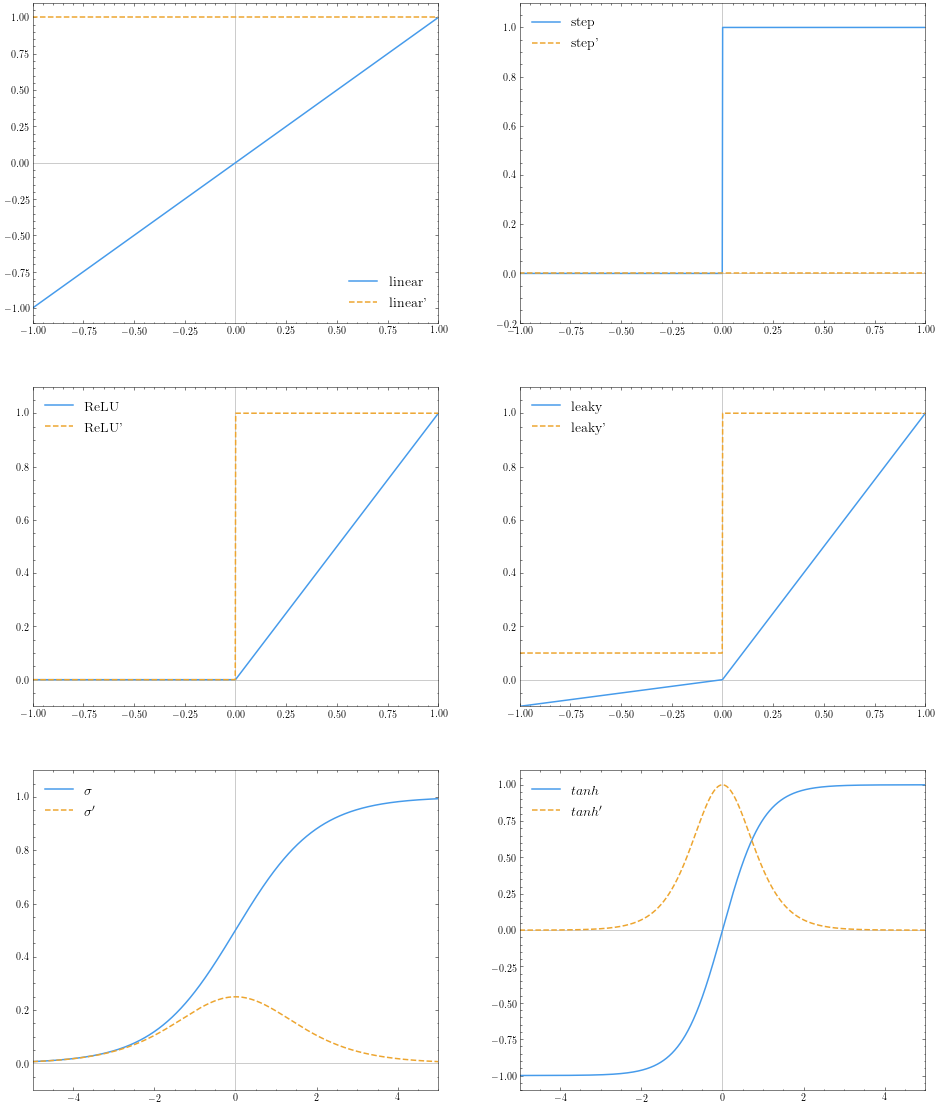
\includegraphics[width=15cm]{images/state-of-art/activation-functions/activation_functions.png}
    \caption{Gráficas de las funciones de activación}
    \label{fig:basicneuron}
\end{figure}

Cada neurona podría tener una función de activación asociada, pero por convención se usa un único tipo de función de activación por cada capa. Ambas soluciones aportan resultados similares y ninguna aporta en principio mejoras significativas al resultado del modelo. La principal diferencia es la complejidad que se añade a la hora de desarrollar una red si se quiere usar una función de activación distinta por neurona. En conclusión, siempre se opta por el uso de una única función de activación en todas las neuronas de una capa por simplicidad de desarrollo. 
\newline
\subsubsection{Trabajando con matrices}\label{workingwithmatrixes}
Para facilitar la explicación a partir de este punto, se procede a explicar distintas partes de la red y su notación matemática con alguna simplificación.
\newline

Se parte de la siguiente definición de red neuronal:

\begin{figure}[H]
    \centering
    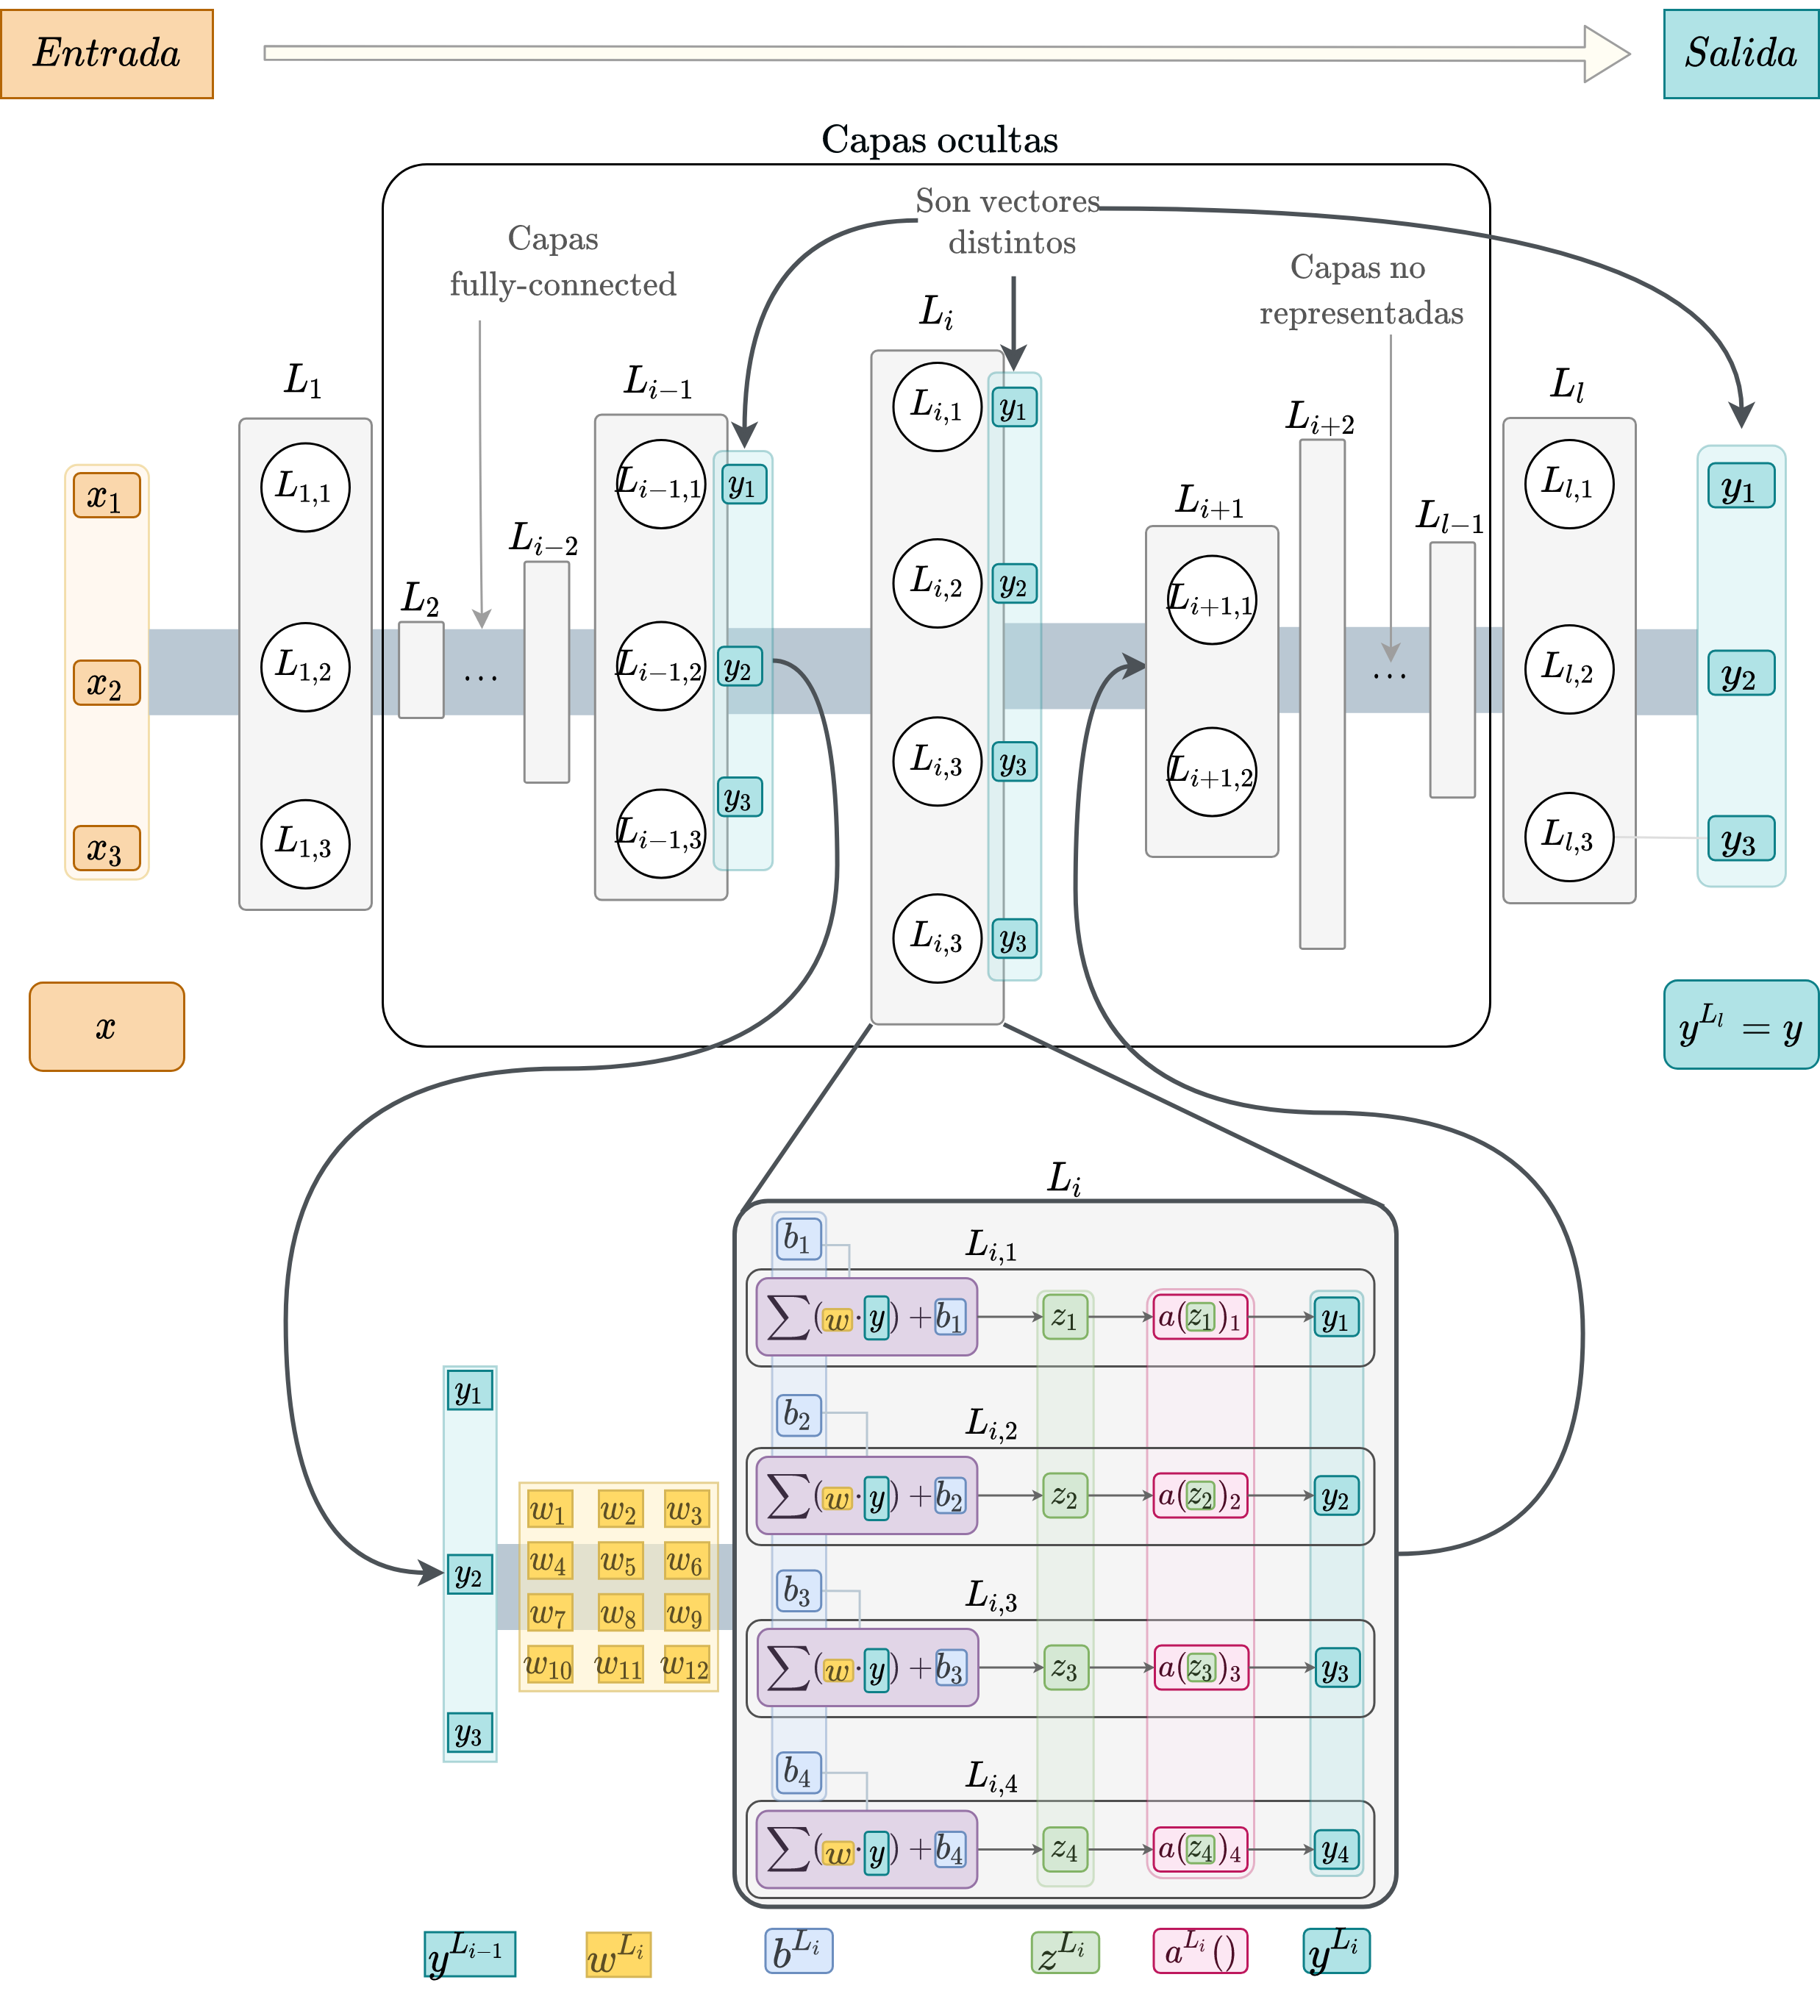
\includegraphics[width=16cm]{images/state-of-art/matrixes/layer_activation_representation.png}
    \caption{Red neuronal}
    \label{fig:basic_network51}
\end{figure}

La red representada necesita cinco valores de entrada que devuelve un único valor, así el modelo será entrenado para que, dado un vector de cinco elementos, el modelo prediga un elemento. El valor que devuelva el modelo será igual al valor $y$, calculado en la última capa:

\begin{equation}
    \begin{split}
    y = a^{L_3}(z_3) &= w_3 \cdot a^{L_2}(z_2) + b_3 \\ 
    \text{donde}~L_i &= \text{Capa número  } i \\
  ~w_j &= \text{Pesos en la capa } j \\ 
  ~b_k &= \text{\textit{Biases} de la capa } k \\
  ~a^{L_{u}}(z_{u}) &= \text{Resultado de la función de activación de la capa } L_{u} \text{ sobre el vector } z_u \\
  ~a^{L_2}(z_2) &= \text{Vector con los valores de la salida de penúltima capa}
  \end{split}
  \label{eqn:layer3}
\end{equation}

El número de elementos de $z_2$ será el mismo número de neuronas que haya en la capa $L_2$. Esto ocurre $\forall z_i$. El vector $z_2$ es calculado en la capa $L_2$ de la siguiente forma:
\begin{equation}
    z_2 = w_2 \cdot a^{L_1}(z_1) + b_2
  \label{eqn:layer2}
\end{equation}

A su vez  $z_1$ viene dado por:
\begin{equation}
    \begin{split}
    z_1 &= w_1 \cdot x + b_1 \\
    \text{donde}~x &= \text{Vector de entrada}
  \end{split}
  \label{eqn:layer1}
\end{equation}

Para hacer referencia a una capa de la red se usará $L_i$, siendo $i$ el índice de la capa ($i=1$ para la primera capa, $i=2$ para la segunda capa...). Para hacer referencia a la última capa, se usará $L_l$, la penúltima será $L_{l-1}$ y así sucesivamente. Se puede añadir un segundo índice para hacer referencia a una neurona tal que $L_{i, j}$ y al igual que el índice de capa, si $j=1$, hará referencia a la primera neurona de la capa, si $j=2$, hará referencia a la segunda neurona de la capa y así respectivamente. A modo de ejemplo la tercera neurona de la segunda capa será referenciada como $L_{2, 3}$ o $L_{l-1, 3}$.
\newline

El vector $w$ y valor $b$ de $L_{2, 3}$ serán referenciados tal que $w^{L_{2,3}}$ y $b^{L_{2,3}}$ respectivamente. Si se quiere hacer referencia a un valor del vector $w$ en concreto se usará un tercer índice tal que $w^{L_{i,j}}_k$. Por ejemplo, $w^{L_{2,3}}_1$ hará referencia al primer peso de la tercera neurona de la segunda capa.
\newline

Sabiendo esta nueva notación, a partir de este punto se simplificarán las ecuaciones. Por ello, los parámetros de una neurona vendrán en un único vector añadiendo el valor $b$ al vector ya existente $w$. Todos los vectores se agruparán formando una matriz $W$, donde cada fila será el vector asociado a una neurona. Es decir, los parámetros de una capa $L_i$ vendrá dado como una matriz a la que se hará referencia como $W$. 

\begin{equation}
\centering
    \begin{split}
    W^{L_i} &= \begin{pmatrix}
  b^{L_{i,1}} & w^{L_{i, 1}}_1 & w^{L_{i, 1}}_2 & \cdots & w^{L_{i, 1}}_n \\
  b^{L_{i,2}} & w^{L_{i, 2}}_1 & w^{L_{i, 2}}_2 & \cdots & w^{L_{i, 2}}_n \\
  b^{L_{i,3}} & w^{L_{i, 3}}_1 & w^{L_{i, 3}}_2 & \cdots & w^{L_{i, 3}}_n \\
  \vdots & \vdots  & \vdots & & \vdots \\
  b^{L_{i,m}} & w^{L_{i, m}}_1 & w^{L_{i, m}}_2 & \cdots & w^{L_{i, m}}_n
  \end{pmatrix} \\ 
    \text{donde}~i &= \text{Índice de la capa en la red} \\
  ~n &= \text{Número de neuronas en }L_{i-1}\text{ o longitud de vector de entrada si } i=1 \\
  ~m &= \text{Número de neuronas en la capa } L_i
  \end{split}
  \label{examplenn51}
\end{equation}

Como ejemplo, la matriz $W^{L-1}$ de la red neuronal definida en la figura \ref{fig:basic_network51} sería la siguiente:

\begin{equation}
  W^{L_{l-1}} = W^{L_2} = \begin{pmatrix}
  b_1 & w_1 & w_2 & w_3 \\
  b_2 & w_4 & w_5 & w_6 \\ 
  b_3 & w_7 & w_8 & w_9 \\ 
  b_4 & w_{10} & w_{11} & w_{12}
  \end{pmatrix} 
  \label{eqn:matrixlayer}
\end{equation}



Usando el ejemplo de la figura \ref{fig:xorgatenetwork}, donde se usan valores específicos para $w$ y $b$, las matrices de cada capa con los parámetros quedarían tal que:

\begin{equation}
  W^{L_1} = \begin{pmatrix}
  0 & 1 & 1 \\ 
  -1 & 1 & 1
  \end{pmatrix}
\end{equation}

\begin{equation}
  W^{L_2} = \begin{pmatrix}
  -2 & 3 & -2
  \end{pmatrix}
\end{equation}

Con esta nueva notación en una sola matriz se recoge los parámetros que necesita calcular la regresión. De hecho, esta matriz es los que el modelo tendrá que "aprender" para obtener mejores resultados. Esto se verá más en detalle en la sección \ref{training}.
\newline

En la ecuación \ref{eqn:activationfunctionbasic} se calculaba el valor con la función $a()$ de la neurona. A partir de este punto, una función de activación recibirá un vector con los valores $z$ de cada neurona y por tanto esta función $a()$ también devolverá un vector del mismo tamaño. En la primera capa de la red, este vector será calculado tal que:
\begin{equation}
  y_1 = a^{L_1}(z) = a(W^{L_1}x)
  \label{eqn:activationmatrixwrong}
\end{equation}

Pero al definir la matriz $W$ de esta forma, el producto $W^{L_1}x$ es imposible de calcular. Esto se puede demostrar usando el ejemplo de la figura \ref{examplenn51}. La dimensión de $W^{L_1}$ es $(3 \times 6)$. Sin embargo, el vector $x$ con el que se va a multiplicar tiene una dimensión $(1 \times 5)$. Para solucionar este problema, se añadirá un $1$ al vector $x$, vector conocido como $x'$ y se realizará la transpuesta de dicho vector. De esta forma se podrá multiplicar la matriz $W$ con dimensión $3\times6$ con un vector de dimensión $6\times1$.

\begin{equation}
\centering
    \begin{split}
  a^L_1(z) &= a(W^{L_2}x') \\
    \text{donde}~x' &= [[1] \oplus x]^T = [1, x_1, x_2, ... x_n]^T \\
    n &= \text{Tamaño del vector } x \\
    A \oplus B &: \text{Concatenación de vectores } A \text{ y } B
  \end{split}
  \label{eqn:newactivationsimple}
\end{equation}

El resto de las capas no tiene este problema. El vector obtenido en la anterior capa ya cumple con las condiciones necesarias para poder realizar el productor de una matriz por un vector. El vector $a^{L_2}(z)$ usará la misma ecuación que \ref{eqn:activationmatrixwrong}, pero la variable $x$ será el vector $y$ calculado en la anterior capa:
\begin{equation}
  a^{L_2}(z) = a(W^{L_2} \cdot a(W^{L_1}x'))
\end{equation}

Se realizará este proceso hasta llegar a la última capa de la red. Se puede leer más información en la sección \ref{feedforward}.
\newline


Actualizando también las ecuaciones \ref{eqn:layer3}, \ref{eqn:layer2} y \ref{eqn:layer1}:
\begin{equation}
    y = a^{L_3}(z_3) = W^{L_3} \cdot a^{L_2}(z_2) 
\end{equation}
\begin{equation}
    z_2 = W^{L_2} \cdot a^{L_1}(z_1)
\end{equation}
\begin{equation}
    z_1 = W^{L_1} \cdot x'
\end{equation}

Agrupando todas las ecuaciones en una sola, el valor de $y$ viene dado por:
\begin{equation}
    y = a(W^{L_3} \cdot (a(W^{L_2} \cdot (a(W^{L_1} \cdot x')^{L_1}))^{L_2}))^{L_3}
    \label{eqn:feedforwardexample}
\end{equation}

Esta ecuación es la que resuelve el modelo para poder obtener el valor $y$ y es lo que se conoce como algoritmo de \textit{feed-forward}.
\newline
\subsubsection{Algoritmo de \textit{feed-forward}}\label{feedforward}
El algoritmo \textit{feed-forward} es el algoritmo básico con el cual una red neuronal predice $y$. Como se ha visto en la ecuación \ref{eqn:feedforwardexample}, el algoritmo es al fin y al cabo una combinación de productos de matrices y funciones de activaciones. Se puede definir una ecuación general de la siguiente forma:

\begin{equation}
    y = a(W^{L_l} \cdot (a(W^{L_{l-1}} \cdot ... \cdot (a(W^{L_1} \cdot x')^{L_1})) \text{ } ... \text{ } ^{L_{l-1}}))^{L_l}
    \label{eqn:feedforward}
\end{equation}

Esta ecuación está computando el algoritmo \textit{feed-forward}, que se resume en los siguientes pasos:

\begin{enumerate}
\item Se tendrá un vector $x$:
\begin{enumerate}
    \item Si es la primera capa del modelo, $x$ es el dado al modelo como argumento de entrada (vector $x$) pero traspuesto.
    \item E.o.c. $x$ vendrá dado calculado por la capa anterior (vector $y$).
\end{enumerate}
\item Se computa $x'$ introduciendo un $1$ en el inicio del vector.
\begin{equation}
  x' = [1] \oplus x
\end{equation}

\item Se calculará $y$:
\begin{equation}
  y = a(Wx')
\end{equation}
\item Si es la última capa, la predicción del modelo será $y$, e.o.c. volver al paso 1.b.
\end{enumerate}

El mismo algoritmo en pseudocódigo:

\begin{algorithm}[H]
\caption{Algoritmo de \textit{feed-forward}}
\SetAlgoLined
\KwResult{Cálculo vector $y$}
 i = 0\;
 n = Número de capas de la red\;
 x = Vector de entrada\;
 y = Vector de salida\;
 \While{$i\neq n$}{
  \eIf{i == 0}{
   $y' = x^T$\;
   }{
   $y' = y$\;
  }
  $x' = [[1] \oplus y']$\;
  $z = W^{L_i}x'$\;
  $y = a^{L_i}(z)$\;
  $i++$\;
 }
\end{algorithm}


Con esta ecuación es fácil ver que el uso de una función de activación por cada capa es necesaria. Como se ha explicado en la sección \ref{activationfunction}, sin el uso de las funciones de activación, un conjunto de capas puede ser compactada en una sola capa. A continuación, se muestra la demostración matemática:
\begin{equation}
\centering
    \begin{split}
    y = W^{L_l} \cdot W^{L_{l-1}} \cdot ... \cdot W^{1} \cdot x' &= (\prod_{l;i-=1}^{i=1} W^{L_i})x' = W'x'\\
    \text{donde}~W' &= (\prod_{l;i-=1}^{i=1} W^{L_i})
  \end{split}
    \label{eqn:feedforwardnoactivation}
\end{equation}

Esta red colapsa a una única capa cuyos parámetros vienen dados por la matriz de $W'$. Usando el ejemplo de la figura \ref{fig:basic_network51}, si se decidiera no usar funciones de activación, la dimensión de la matriz $W'$ sería de $(3,1)$ que coincide con el tamaño del vector de entrada($x$) y el tamaño del vector de salida($y$).

\begin{equation}
\centering
    \begin{split}
    dim(W^1&) = (3,6) \\
    dim(W^2&) = (6,5) \\
    dim(W^3&) = (5,1) \\ \\
    dim(W^1 &\cdot W^2) = (3,5)\\
    dim(W') &= dim(W^1 \cdot W^2 \cdot W^3) = (3,1)
    \end{split}
\end{equation}

Recordando la siguiente regla para el producto de matrices para un producto de matrices $A \times B = C$:

\begin{equation}
\centering
    \begin{split}
    dim(A) &= (m, n) \\
    dim(B) &= (n, k) \\
    dim(C) &= (m, k)
    \end{split}
    \label{eqn:dimensions}
\end{equation}

\begin{itemize}
    \item La dimensión de la matriz $C$ viene dada por el número de filas de $A$, $m$, y el número de columnas de $B$, $n$.
    \item El número de columnas de $A$($m$) debe coincidir con el número de columnas de $B$($n$)
    , condición que se cumple puesto que se está trabajando con redes neuronales \textit{fully-connected}, todas las neuronas de una capa están conectadas a las neuronas de la siguiente capa.
\end{itemize}

Volviendo a la ecuación \ref{eqn:feedforwardnoactivation} y realizando el mismo cálculo que se ha realizado en la ecuación \ref{eqn:dimensions} sobre la red que se quiera, se puede obtener el tamaño de $y$ que será calculada por el modelo. El número de filas indicará el número de datos que se han predicho y el número de columnas es el número de etiquetas por cada dato.
\newline

En la red mostrada en la figura \ref{fig:basic_network51}, tiene como entrada cinco variables. A modo de ejemplo, se podría usar esta red para crear el modelo del siguiente problema: Predecir el coste de una vivienda en una ciudad dado un conjunto de datos de vivienda en esa misma ciudad. Se quiere predecir el valor del precio a partir de las siguientes variables: número de habitaciones, tipo de vivienda, porcentaje de criminalidad, coordenadas geográficas y metros cuadrados. Esto se puede representar como una tabla donde cada fila es una vivienda.
\newline


\begin{table}[H]
  \centering
  \begin{threeparttable}[t]
       \begin{tabular}{l|llrrrr}
        \toprule
        {} &   \textbf{tipo} & \textbf{coords} & \textbf{gc$^1$} & \textbf{m2$^2$} &  \textbf{h$^3$} & \textbf{precio} \\
        \midrule
        \textbf{1} &       Estudio &  $(40.35717, -3.81053)$ &   $5$ &   $41$ & $2$ &  65.378 \\
        \textbf{2} &   Apartamento &  $(40.53125, -3.72054)$ &   $2$ &   $49$ &  $3$ & 79.519 \\
        \textbf{3} &        Dúplex & $(40.45990, -3.60053)$  &   $5$ &   $59$ &  $3$ & 82.578 \\
        \textbf{4} &   Apartamento &  $(40.43437, -3.74870)$ &   $1$ &   $84$ &  $3$ & 99.701 \\
        \textbf{5} &   Apartamento &  $(40.43646, -3.84071)$ &   $3$ &  $100$ & $5$ & 130.978 \\
        \textbf{6} &         Chalé &  $(40.41922, -3.57909)$ &   $1$ &  $126$ & $6$ & 160.890 \\
        \textbf{7} &   Apartamento &  $(40.47372, -3.58115)$ &   $4$ &   $94$ & $4$ & 215.000 \\
        \textbf{8} &         Ático &  $(40.52186, -3.57051)$ &   $4$ &  $142$ & $6$ & 285.398 \\
        \textbf{9} &         Chalé &  $(40.44979, -3.68003)$ &   $3$ &  $185$ & $7$ & 340.589 \\
        \textbf{10} &       Dúplex & $(40.49347, -3.67969)$ & $2$ &  $209$ & $8$ & 426.000 \\
        \bottomrule
         \end{tabular}
     \begin{tablenotes}
     \item[1] gc: Grado de criminalidad del barrio.
     \item[2] m2: metros cuadrados.
     \item[3] h: Número de habitaciones.
   \end{tablenotes}
    \end{threeparttable}%
  \label{tab:houses}%
\caption{Ejemplo de \textit{dataset} con viviendas}
\end{table}%



% TODO Tabla

%La predicción del valor de una vivienda se calculará a partir de cinco variables de entrada. % Por cada vivienda que se quiera estudiar, se tendrá cinco valores con los que trabajar.

